\documentclass[a4paper,german,12pt,smallheadings]{scrartcl}
\usepackage[T1]{fontenc}
\usepackage[utf8]{inputenc}
\usepackage{babel}
\usepackage{geometry}
\usepackage{pdfpages}
\usepackage{tikz}
\usetikzlibrary{calc,intersections,fadings}
\usepackage{wrapfig}
\usepackage[fleqn]{amsmath}
\usepackage{amssymb}
\usepackage{float}
\usepackage{enumerate}
\usepackage{listings} % Source code
\usepackage{lscape} % landscape
\usepackage{commath} % http://tex.stackexchange.com/questions/14821/whats-the-proper-way-to-typeset-a-differential-operator
\usepackage{cancel}
\usepackage[fleqn]{mathtools}
% Number only referenced equations
%\mathtoolsset{showonlyrefs}

%\usepackage{wrapfig}
\usepackage{siunitx}
\sisetup{separate-uncertainty=true,locale=DE}

% http://tex.stackexchange.com/questions/38818/best-way-to-denote-an-angle-in-tikz
\newcommand\markangle[6][red]{% [color] {X} {origin} {Y} {mark} {radius}
  % filled circle: red by default
  \begin{scope}
    \path[clip] (#2) -- (#3) -- (#4);
    \fill[color=#1,fill opacity=0.5,draw=#1,name path=circle]
    (#3) circle (#6mm);
  \end{scope}
  % middle calculation
  \path[name path=line one] (#3) -- (#2);
  \path[name path=line two] (#3) -- (#4);
  \path[%
  name intersections={of=line one and circle, by={inter one}},
  name intersections={of=line two and circle, by={inter two}}
  ] (inter one) -- (inter two) coordinate[pos=.5] (middle);
  % bissectrice definition
  \path[%
  name path=bissectrice
  ] (#3) -- (barycentric cs:#3=-1,middle=1.2);
  % put mark
  \path[
  name intersections={of=bissectrice and circle, by={middleArc}}
  ] (#3) -- (middleArc) node[pos=1.3] {#5};
  }

% New command for color underlining
\usepackage{xcolor}
\newcommand\invisiblesection[1]{%
    \refstepcounter{section}%
      \addcontentsline{toc}{section}{\protect\numberline{\thesection}#1}%
        \sectionmark{#1}}
\newsavebox\MBox
\newcommand\colul[2][red]{{\sbox\MBox{$#2$}%
  \rlap{\usebox\MBox}\color{#1}\rule[-1.2\dp\MBox]{\wd\MBox}{0.5pt}}}

\restylefloat{table}
\geometry{a4paper, top=15mm, left=20mm, right=10mm, bottom=20mm, headsep=10mm, footskip=12mm}
\linespread{1.5}
\setlength\parindent{0pt}
\DeclareMathOperator{\Tr}{Tr}
\DeclareMathOperator{\Var}{Var}
\begin{document}

\begin{titlepage}
\newcommand{\HRule}{\rule{\linewidth}{0.5mm}}

\begin{center}
  \textsc{\Large Physikalisches Grundpraktkum 1}
  \HRule\\[0.4 cm]
  {\huge \bfseries Gleichmäßig beschleunigte Drehbewegungen}
  \HRule\\[0.4 cm]

  \begin{minipage}{0.65\textwidth}
  \begin{flushleft}
    Markus Fenske \texttt{<iblue@zedat.fu-berlin.de>} \\
    Paul Rahmann \texttt{<paulrahmann@zedat.fu-berlin.de>}
  \end{flushleft}
  \end{minipage}
  \hfill
  \begin{minipage}{0.30\textwidth}
  \begin{flushright}
    Tutor: Christian Hindermann \\
    Versuchstag: 6. Juni 2014
  \end{flushright}
  \end{minipage}

  \vspace{1cm}

  \tableofcontents


  %{\large \today}
  \vfill
\end{center}
\newpage

\end{titlepage}

\allowdisplaybreaks % Seitenumbrüche in Formeln erlauben

\section{Physikalische Grundlagen}
\subsection{$\gamma$-Strahlung}

Beim Zerfall von instabilen Atomkernen gibt es, neben anderen Möglichkeiten,
zwei Hauptzerfallskanäle. Beim $\alpha$-Zerfall, stößt der Mutterkern
$\mathrm{X}$ einen Helium-4-Kern, bestehtend aus zwei Protonen und zwei
Neutronen, aus.  Entsprechend hat der Tochterkern $\mathrm{Y}$ eine um vier
verringerte Massenzahl und eine um zwei verringerte Kernladungszahl.

\begin{equation}
  {}^{A}_{Z} \mathrm{X} \to {}^{A-4}_{Z-2} \mathrm{Y} + {}^{4}_{2} \mathrm{He}
\end{equation}

Die freiwerdende Energie führt zu einer kinetischen Energie der beiden Kerne,
regt aber in der Regel auch den entstehenden Tochterkern an.

Beim $\beta^{-}$-Zerfall wird im Mutterkern ein Neutron in ein Proton, ein
Elektron und ein Anti-Elektron-Neutrino umgewandelt.

\begin{equation}
  \mathrm{n} \to \mathrm{p} + \mathrm{e}^{-} + \overline{\nu}_e
\end{equation}

Die Kernladungszahl erhöht sich dabei um eins, die Massenzahl bleibt konstant.

Auch hierbei wird Energie frei, die in die kinetische Energie des Elektrons und
des Anti-Neutrinos fließt, aber auch in eine Kernanregung des Tocherkerns.

Es existieren weitere Zerfallskanäle wie $\beta^+$-Zerfall, spontane Fission
oder auch Emission von Protonen odr Neutronen bei sehr kurzlebigen Isotopen,
die aber hier nicht relevant sind.

Die Kernanregung führt in der Regel zu einer Kernspin-Anregung, die dann als
elektromagnetische Multipolstrahlung relaxiert. Die entstehenden Photonen nennt
man aus historischen Gründen $\gamma$-Strahlung. Sie können mit der Hülle des
entsprechenden Atoms wechselwirken (innere Konversion, IC). Dabei überträgt ein
$\gamma$-Quant einen Teil seiner Energie an ein Hüllenelektron. Die
resultierende kinetische Energie des Elektrons ergibt sich aus der Differenz zu
seiner Bindungsenergie.

\begin{equation}
  E_e = E_\gamma - E_B
\end{equation}

Gegenstand unseres Experiments ist der qualitative und quantitative Nachweis
von $\gamma$-Strahlung.

\subsection{Nachweis von $\gamma$-Strahlung}

Zum Nachweis von $\gamma$-Strahlung nutzt man die Wechselwirkung der Photonen
mit Materie (siehe unten). Es gibt dabei zwei Hauptmöglichkeiten.

In einem Szintillationsdetektor werden die Atome bzw. Moleküle eines Stoffes
(in der Regel ein Festkörper im klassischen Sinne) durch die $\gamma$-Quanten
angeregt. Die Relaxation führt dann zur Abstrahlung von Photonen geringerer
Energie (in der Regel im sichtbaren Bereich), die dann aufgefangen und gemessen
werden können (z.B. per Photomultiplier).

Bei einem Halbleiterdetektor handelt es sich, vereinfacht ausgedrückt, um eine
in Sperrrichtung betriebende, elektronische Diode, sodass trotz angelegter
Spannung kein Strom fließt. Trifft nun ein $\gamma$-Quant auf, wird im
Halbleitermaterial ein Elektron-Loch-Paar erzeugt, die dann aufgrund des
anliegenden elektrischen Feldes zu den Anschlussdrähten wandern und dadurch
einen Strom-Impuls erzeugen, der messbar ist.

Bei beiden Detektoren deponiert das $\gamma$-Quant nicht zwangsläufig seine
gesamte Energie auf einmal, sodass selbst monochromatische $\gamma$-Strahlung
zu einer Energieverteilung der Elektronen führt.

Zur Charakterisierung des entstehenden Spektrums benutzt man daher die Begriffe
\textit{Photopeak}, \textit{Compton-Spektrum} und \textit{Escape-Peak}.

% ??? Ist das korrekt ???
Der Photopeak tritt dort auf, wo das $\gamma$-Quant seine gesamte Energie
deponiert, er tritt als schmaler Ausschlag hervor. Das Compton-Spektrum ist das
sich daran anschließende Kontinuum, das der Verteilung des Compton-Effekts
entspricht. Escape-Peaks sind Messartefakte, die durch verschiedene Effekte
innerhalb des Detektormaterials entstehen und mit Photopeaks verwechselt werden
können.

\subsection{Wechselwirkung von $\gamma$-Strahlung mit Materie}

\subsubsection{Photoeffekt}

Beim Photoeffekt werden durch die Strahlung Atome im Detektormaterial
ionisiert. Diese werden durch andere Elektronen ersetzt, möglicherweise auch in
mehreren Schritten, wobei Röntgenstrahlung emmitiert wird, die auch wieder vom
Detektor absorbiert wird. Auch ein Auger-Prozess ist möglich. Bei diesem werden
Elektronen emmitiert, deren kinetische Energie aber auch wieder photonisch
umgewandelt und dann detektiert wird. Da die gesamte Energie also im
Detektormaterial als Photonen abgestrahlt wird, verfälscht dieser Prozess das
Messergebnis nicht.

\subsubsection{Compton-Effekt}

Beim Compton-Effekt stößt ein hochenergetisches Photon an quasi-freien Elektron
(quasi-frei, weil die Bindungsenergie sehr viel kleiner als die Energie des
Photons ist). Zur Herleitung:

Seien $p_\gamma$ und $p_\gamma'$ die 4-Impulse der Photonen vor und nach dem
Stoß und seien $p_e$ und $p_e'$ die 4-Impulse der Elektronen vor und nach dem
Stoß, dann gilt aufgrund der 4-Impuls-Erhaltung

\begin{align}
  &p_\gamma + p_e = p_\gamma' + p_e' \\
  \Leftrightarrow\quad & (p_\gamma - p_\gamma')^2 = (p_e' - p_e)^2 \\
  \Leftrightarrow\quad & p_\gamma^2 - 2p_\gamma p_\gamma' - p_\gamma^2 = p_e'^2 - 2p_ep_e' + p_e'^2
\end{align}

Wir können das Bezugssystem frei wählen und wählen daher das Ruhesystem des
Elektrons vor dem Stoß, also ist $p_\gamma = (E_\gamma/c, \vec{p_\gamma})$,
$p_\gamma' = (E_\gamma'/c, \vec{p_\gamma'})$, $p_e = (m_e c, \vec{0})$, $p_e' =
(E_e'/c, \vec{p_e}')$. Somit

\begin{align}
  \Leftrightarrow\quad&-2\left(\frac{E_\gamma E_\gamma'}{c^2} - \vec{p_\gamma} \cdot \vec{p_\gamma}'\right) = 2m_e^2c^2 - 2 m_e E_e'
\end{align}

Mit dem Kosinussatz (sei $\phi$ der Winkel zwischen den photonischen
3-Impulsen) und der Energiegieerhaltung $E_e' = m_ec^2 + (E_\gamma -
E_\gamma')$, sowie $E = pc$ für Photonen folgt

\begin{align}
  \Leftrightarrow\quad&\frac{E_\gamma E_\gamma'}{c^2}(1 - \cos \phi) = m_e(E_\gamma - E_\gamma') \\
  \Leftrightarrow\quad&\frac{E_\gamma E_\gamma'}{m_e c^2}(1 - \cos \phi) + E_\gamma' = E_\gamma \\
  \Leftrightarrow\quad&E_\gamma' \left(\frac{E_\gamma}{m_e c^2}(1 - \cos \phi) + 1\right) = E_\gamma \\
  \Leftrightarrow\quad&E_\gamma' = \frac{E_\gamma}{1 + \frac{E_\gamma}{m_e c^2}(1 - \cos \phi)}
\end{align}

Man sieht hier, dass die deponierte Energie $E_\gamma - E_\gamma'$ ab größten
ist, wenn sich der Winkel $\phi$ einer Reflexion ($180^\circ$) entspricht. Für
kleine Winkel $\phi \approx 0$ findet kein Energieübertrag statt.

Durch den Compton-Effekt ist es möglich, dass das Photon den Detektor verlässt
(durch Reflexion), bevor die Energie vollständig deponiert wurde. Dadurch
entstehen Linien geringerer Energie, die wir Backscatter-Linien nennen.

\subsubsection{Paarbildung}

Ab photonischen Energien, die dem doppelten der Ruheenergie des Elektrons
entsprechen, entstehen Elektron-Positron-Paare. Die Energie kann durch
Anihilation zurückgewonnen werden und wird dann wieder in Form von Photonen
abstrahlt und detektiert. Verlässt jedoch eines oder beide der Teilchen den
Detektor, verringert sich die detektierte Energie um die Ruhemasse bzw. deren
Summe (heißt 511 keV (Single-Escape-Peak) bzw. 1022 keV (Double-Escape-Peak)).

\subsection{Verwendete Geräte}

Wir verwenden einen NaI(Tl)-Szintillationsdetektorkristall, dessen erzeugte
Photonen mithilfe eines Photomultipliers detektiert werden (Funktionsweise
siehe oben). Die Energieauflösung dieses Detektors liegt ungefähr eine
Größenordnung unter der, des Halbleiterdetektors.

Außerdem verwenden wir einen Ge-Halbleiterdektor (Funktionsweise siehe oben).

Die Signale der beiden Detektoren werden mit einem Vorverstärker integriert und
in Impulse umgeformt, deren Höhen proportional zur Ladung des Detektorpulses
sind. Im angeschlossenen Hauptverstärker werden die Impulse geformt und
gefiltert und dann mit einem Vielkanalanalysator analysiert. Der
Vielkanalanlysator trägt dazu die Häufigkeit der Signale über ihrer Höhe auf.

\section{Auswertung}

\subsection{Aufgabe 1}

Zur Aufnahme der Impulsformen und Zeiten und deren Diskussion siehe Messprotokoll.

\subsection{Aufgabe 2}

Da die Kanalzahl proportional zur Energie ist, ergibt sich die Energieauflösung
durch die Division der Kanalbreite (Full Width 1/5 Maximum) durch die Kanalzahl.

\begin{equation}
  \frac{\Delta E}{E_\text{exp}} = \frac{\text{FW(1/5)M (Kanalzahl)}}{\text{Peak (Kanalzahl)}}
\end{equation}

\begin{tabular}{l|l}
  Linie & relvative Energieauflösung ($\Delta E/E_\text{exp}$) \\
  \hline
  Co-60 1{,}33 MeV & 0{,}082 \\
  Co-60 1{,}17 MeV & 0{,}079 \\
  Na-22 1{,}27 MeV & 0{,}054 \\
  Cs-137 661 keV & 0{,}134 \\
\end{tabular}
\vspace{22pt}

Die lineare Regression zur Bestimmung des Eichfaktors befindet sich weiter
hinten. Man sieht, dass die Energieeichung trotz der breiten Peaks genau
möglich ist. Der Eichfaktor wurde zu $m = 4591\pm53$ bestimmt, dies entspricht
der Kanalzahl der 1-MeV-Energie.

\subsection{Aufgabe 3}

TODO.

\subsection{Aufgabe 4}

Zur Aufnahme der Impulsformen und Zeiten und deren Diskussion siehe Messprotokoll.

\subsection{Aufgabe 5}

Die Energieauflösung wurde analog zu Aufgabe 2 bestimmt.

\begin{tabular}{l|l|l}
  Linie & relvative Energieauflösung ($\Delta E/E_\text{exp}$) & Verhältnis zu NaI \\
  \hline
  Co-60 1{,}33 MeV & 0{,}015 & 0{,}18\\
  Co-60 1{,}17 MeV & 0{,}011 & 0{,}13\\
  Na-22 1{,}27 MeV & 0{,}010 & 0{,}18\\
  Cs-137 661 keV & 0{,}017 & 0{,}13\\
  Am-241 26 keV & 0{,}57 \\
  Am-241 60 keV & 0{,}057
\end{tabular}
\vspace{22pt}

Man sieht, dass die Energieauflösung des Halbleiterdetektors knapp eine
Größenordnung besser ist, als die Energieauflösung des Szintillationsdetektors,
wie in der Versuchsanleitung angegeben.

Die Energieeichung des Halbleiterdetektors führt zu einem Eichfaktor von $m =
4597\pm25$ (Kanalzahl der 1-MeV-Linie).


\subsection{Aufgabe 6}

TODO.

\subsection{Aufgabe 7}

TODO.

\begin{landscape}
  % GNUPLOT: LaTeX picture with Postscript
\begingroup
  \makeatletter
  \providecommand\color[2][]{%
    \GenericError{(gnuplot) \space\space\space\@spaces}{%
      Package color not loaded in conjunction with
      terminal option `colourtext'%
    }{See the gnuplot documentation for explanation.%
    }{Either use 'blacktext' in gnuplot or load the package
      color.sty in LaTeX.}%
    \renewcommand\color[2][]{}%
  }%
  \providecommand\includegraphics[2][]{%
    \GenericError{(gnuplot) \space\space\space\@spaces}{%
      Package graphicx or graphics not loaded%
    }{See the gnuplot documentation for explanation.%
    }{The gnuplot epslatex terminal needs graphicx.sty or graphics.sty.}%
    \renewcommand\includegraphics[2][]{}%
  }%
  \providecommand\rotatebox[2]{#2}%
  \@ifundefined{ifGPcolor}{%
    \newif\ifGPcolor
    \GPcolorfalse
  }{}%
  \@ifundefined{ifGPblacktext}{%
    \newif\ifGPblacktext
    \GPblacktexttrue
  }{}%
  % define a \g@addto@macro without @ in the name:
  \let\gplgaddtomacro\g@addto@macro
  % define empty templates for all commands taking text:
  \gdef\gplbacktext{}%
  \gdef\gplfronttext{}%
  \makeatother
  \ifGPblacktext
    % no textcolor at all
    \def\colorrgb#1{}%
    \def\colorgray#1{}%
  \else
    % gray or color?
    \ifGPcolor
      \def\colorrgb#1{\color[rgb]{#1}}%
      \def\colorgray#1{\color[gray]{#1}}%
      \expandafter\def\csname LTw\endcsname{\color{white}}%
      \expandafter\def\csname LTb\endcsname{\color{black}}%
      \expandafter\def\csname LTa\endcsname{\color{black}}%
      \expandafter\def\csname LT0\endcsname{\color[rgb]{1,0,0}}%
      \expandafter\def\csname LT1\endcsname{\color[rgb]{0,1,0}}%
      \expandafter\def\csname LT2\endcsname{\color[rgb]{0,0,1}}%
      \expandafter\def\csname LT3\endcsname{\color[rgb]{1,0,1}}%
      \expandafter\def\csname LT4\endcsname{\color[rgb]{0,1,1}}%
      \expandafter\def\csname LT5\endcsname{\color[rgb]{1,1,0}}%
      \expandafter\def\csname LT6\endcsname{\color[rgb]{0,0,0}}%
      \expandafter\def\csname LT7\endcsname{\color[rgb]{1,0.3,0}}%
      \expandafter\def\csname LT8\endcsname{\color[rgb]{0.5,0.5,0.5}}%
    \else
      % gray
      \def\colorrgb#1{\color{black}}%
      \def\colorgray#1{\color[gray]{#1}}%
      \expandafter\def\csname LTw\endcsname{\color{white}}%
      \expandafter\def\csname LTb\endcsname{\color{black}}%
      \expandafter\def\csname LTa\endcsname{\color{black}}%
      \expandafter\def\csname LT0\endcsname{\color{black}}%
      \expandafter\def\csname LT1\endcsname{\color{black}}%
      \expandafter\def\csname LT2\endcsname{\color{black}}%
      \expandafter\def\csname LT3\endcsname{\color{black}}%
      \expandafter\def\csname LT4\endcsname{\color{black}}%
      \expandafter\def\csname LT5\endcsname{\color{black}}%
      \expandafter\def\csname LT6\endcsname{\color{black}}%
      \expandafter\def\csname LT7\endcsname{\color{black}}%
      \expandafter\def\csname LT8\endcsname{\color{black}}%
    \fi
  \fi
  \setlength{\unitlength}{0.0500bp}%
  \begin{picture}(15306.00,10204.00)%
    \gplgaddtomacro\gplbacktext{%
      \csname LTb\endcsname%
      \put(1210,704){\makebox(0,0)[r]{\strut{} 0}}%
      \put(1210,1628){\makebox(0,0)[r]{\strut{} 5000}}%
      \put(1210,2551){\makebox(0,0)[r]{\strut{} 10000}}%
      \put(1210,3475){\makebox(0,0)[r]{\strut{} 15000}}%
      \put(1210,4398){\makebox(0,0)[r]{\strut{} 20000}}%
      \put(1210,5322){\makebox(0,0)[r]{\strut{} 25000}}%
      \put(1210,6245){\makebox(0,0)[r]{\strut{} 30000}}%
      \put(1210,7169){\makebox(0,0)[r]{\strut{} 35000}}%
      \put(1210,8092){\makebox(0,0)[r]{\strut{} 40000}}%
      \put(1210,9016){\makebox(0,0)[r]{\strut{} 45000}}%
      \put(1210,9939){\makebox(0,0)[r]{\strut{} 50000}}%
      \put(1342,484){\makebox(0,0){\strut{} 0}}%
      \put(3992,484){\makebox(0,0){\strut{} 200}}%
      \put(6642,484){\makebox(0,0){\strut{} 400}}%
      \put(9291,484){\makebox(0,0){\strut{} 600}}%
      \put(11941,484){\makebox(0,0){\strut{} 800}}%
      \put(14591,484){\makebox(0,0){\strut{} 1000}}%
      \put(176,5321){\rotatebox{-270}{\makebox(0,0){\strut{}Intensität [arbiträre Einheiten]}}}%
      \put(8125,154){\makebox(0,0){\strut{}Position [Pixel]}}%
      \put(2292,9662){\makebox(0,0)[l]{\strut{}Aufgabe 5.4}}%
      \put(2292,9442){\makebox(0,0)[l]{\strut{}Fitgleichung: Summe von}}%
      \put(2292,9222){\makebox(0,0)[l]{\strut{}Quadratischem Hintergrund $ax^2+bx+c$ mit $a=0.00734$, $b=-7.26$, $c=4370.0$}}%
      \put(2292,9002){\makebox(0,0)[l]{\strut{}Lorentzian $a/(1+((x-p)/(f/2))^2)$ jeweils mit:}}%
      \put(2292,8782){\makebox(0,0)[l]{\strut{}$p=61.59$, $a=43480.0$, $f=-15.82$}}%
      \put(2292,8562){\makebox(0,0)[l]{\strut{}$p=295.4$, $a=27790.0$, $f=86.86$}}%
      \put(2292,8342){\makebox(0,0)[l]{\strut{}$p=530.2$, $a=37690.0$, $f=17.21$}}%
      \put(2292,8122){\makebox(0,0)[l]{\strut{}$p=631.2$, $a=31100.0$, $f=16.41$}}%
      \put(2292,7902){\makebox(0,0)[l]{\strut{}$p=710.2$, $a=24500.0$, $f=11.73$}}%
      \put(2292,7682){\makebox(0,0)[l]{\strut{}$p=775.3$, $a=20580.0$, $f=10.91$}}%
      \put(2292,7462){\makebox(0,0)[l]{\strut{}$p=832.6$, $a=17310.0$, $f=10.54$}}%
      \put(2292,7242){\makebox(0,0)[l]{\strut{}$p=884.5$, $a=14970.0$, $f=9.653$}}%
      \put(2292,7022){\makebox(0,0)[l]{\strut{}$p=931.9$, $a=13240.0$, $f=8.975$}}%
      \put(2292,6802){\makebox(0,0)[l]{\strut{}$p=976.0$, $a=11280.0$, $f=8.229$}}%
      \put(2292,6582){\makebox(0,0)[l]{\strut{}$p=1018.0$, $a=9241.0$, $f=8.559$}}%
    }%
    \gplgaddtomacro\gplfronttext{%
    }%
    \gplbacktext
    \put(0,0){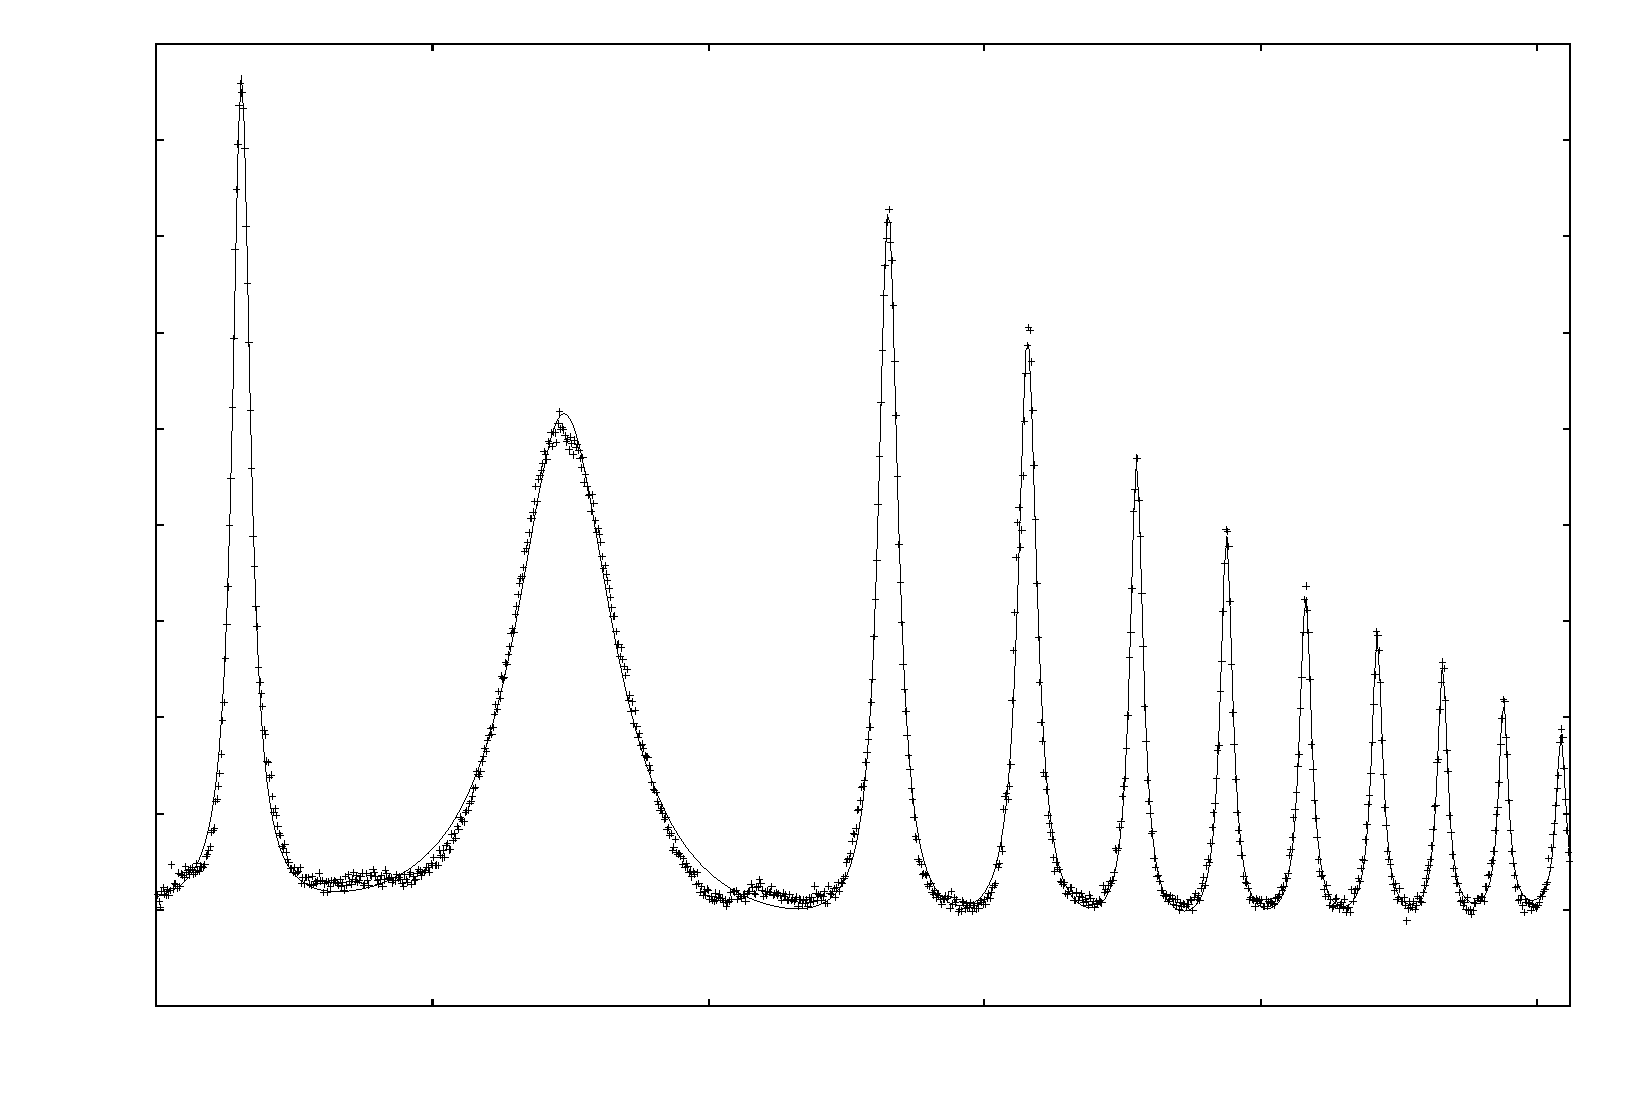
\includegraphics{plot-1}}%
    \gplfronttext
  \end{picture}%
\endgroup

\end{landscape}
\begin{landscape}
  % GNUPLOT: LaTeX picture with Postscript
\begingroup
  \makeatletter
  \providecommand\color[2][]{%
    \GenericError{(gnuplot) \space\space\space\@spaces}{%
      Package color not loaded in conjunction with
      terminal option `colourtext'%
    }{See the gnuplot documentation for explanation.%
    }{Either use 'blacktext' in gnuplot or load the package
      color.sty in LaTeX.}%
    \renewcommand\color[2][]{}%
  }%
  \providecommand\includegraphics[2][]{%
    \GenericError{(gnuplot) \space\space\space\@spaces}{%
      Package graphicx or graphics not loaded%
    }{See the gnuplot documentation for explanation.%
    }{The gnuplot epslatex terminal needs graphicx.sty or graphics.sty.}%
    \renewcommand\includegraphics[2][]{}%
  }%
  \providecommand\rotatebox[2]{#2}%
  \@ifundefined{ifGPcolor}{%
    \newif\ifGPcolor
    \GPcolorfalse
  }{}%
  \@ifundefined{ifGPblacktext}{%
    \newif\ifGPblacktext
    \GPblacktexttrue
  }{}%
  % define a \g@addto@macro without @ in the name:
  \let\gplgaddtomacro\g@addto@macro
  % define empty templates for all commands taking text:
  \gdef\gplbacktext{}%
  \gdef\gplfronttext{}%
  \makeatother
  \ifGPblacktext
    % no textcolor at all
    \def\colorrgb#1{}%
    \def\colorgray#1{}%
  \else
    % gray or color?
    \ifGPcolor
      \def\colorrgb#1{\color[rgb]{#1}}%
      \def\colorgray#1{\color[gray]{#1}}%
      \expandafter\def\csname LTw\endcsname{\color{white}}%
      \expandafter\def\csname LTb\endcsname{\color{black}}%
      \expandafter\def\csname LTa\endcsname{\color{black}}%
      \expandafter\def\csname LT0\endcsname{\color[rgb]{1,0,0}}%
      \expandafter\def\csname LT1\endcsname{\color[rgb]{0,1,0}}%
      \expandafter\def\csname LT2\endcsname{\color[rgb]{0,0,1}}%
      \expandafter\def\csname LT3\endcsname{\color[rgb]{1,0,1}}%
      \expandafter\def\csname LT4\endcsname{\color[rgb]{0,1,1}}%
      \expandafter\def\csname LT5\endcsname{\color[rgb]{1,1,0}}%
      \expandafter\def\csname LT6\endcsname{\color[rgb]{0,0,0}}%
      \expandafter\def\csname LT7\endcsname{\color[rgb]{1,0.3,0}}%
      \expandafter\def\csname LT8\endcsname{\color[rgb]{0.5,0.5,0.5}}%
    \else
      % gray
      \def\colorrgb#1{\color{black}}%
      \def\colorgray#1{\color[gray]{#1}}%
      \expandafter\def\csname LTw\endcsname{\color{white}}%
      \expandafter\def\csname LTb\endcsname{\color{black}}%
      \expandafter\def\csname LTa\endcsname{\color{black}}%
      \expandafter\def\csname LT0\endcsname{\color{black}}%
      \expandafter\def\csname LT1\endcsname{\color{black}}%
      \expandafter\def\csname LT2\endcsname{\color{black}}%
      \expandafter\def\csname LT3\endcsname{\color{black}}%
      \expandafter\def\csname LT4\endcsname{\color{black}}%
      \expandafter\def\csname LT5\endcsname{\color{black}}%
      \expandafter\def\csname LT6\endcsname{\color{black}}%
      \expandafter\def\csname LT7\endcsname{\color{black}}%
      \expandafter\def\csname LT8\endcsname{\color{black}}%
    \fi
  \fi
  \setlength{\unitlength}{0.0500bp}%
  \begin{picture}(15306.00,10204.00)%
    \gplgaddtomacro\gplbacktext{%
      \csname LTb\endcsname%
      \put(946,704){\makebox(0,0)[r]{\strut{} 0}}%
      \put(946,1628){\makebox(0,0)[r]{\strut{} 0.1}}%
      \put(946,2551){\makebox(0,0)[r]{\strut{} 0.2}}%
      \put(946,3475){\makebox(0,0)[r]{\strut{} 0.3}}%
      \put(946,4398){\makebox(0,0)[r]{\strut{} 0.4}}%
      \put(946,5322){\makebox(0,0)[r]{\strut{} 0.5}}%
      \put(946,6245){\makebox(0,0)[r]{\strut{} 0.6}}%
      \put(946,7169){\makebox(0,0)[r]{\strut{} 0.7}}%
      \put(946,8092){\makebox(0,0)[r]{\strut{} 0.8}}%
      \put(946,9016){\makebox(0,0)[r]{\strut{} 0.9}}%
      \put(946,9939){\makebox(0,0)[r]{\strut{} 1}}%
      \put(1078,484){\makebox(0,0){\strut{} 10}}%
      \put(4536,484){\makebox(0,0){\strut{} 100}}%
      \put(7994,484){\makebox(0,0){\strut{} 1000}}%
      \put(11451,484){\makebox(0,0){\strut{} 10000}}%
      \put(14909,484){\makebox(0,0){\strut{} 100000}}%
      \put(176,5321){\rotatebox{-270}{\makebox(0,0){\strut{}$U_R/U_0$}}}%
      \put(7993,154){\makebox(0,0){\strut{}$f$ [Hz]}}%
    }%
    \gplgaddtomacro\gplfronttext{%
      \csname LTb\endcsname%
      \put(13922,9766){\makebox(0,0)[r]{\strut{}Hochpass}}%
      \csname LTb\endcsname%
      \put(13922,9546){\makebox(0,0)[r]{\strut{}Tiefbass}}%
      \csname LTb\endcsname%
      \put(13922,9326){\makebox(0,0)[r]{\strut{}Bandpass}}%
    }%
    \gplbacktext
    \put(0,0){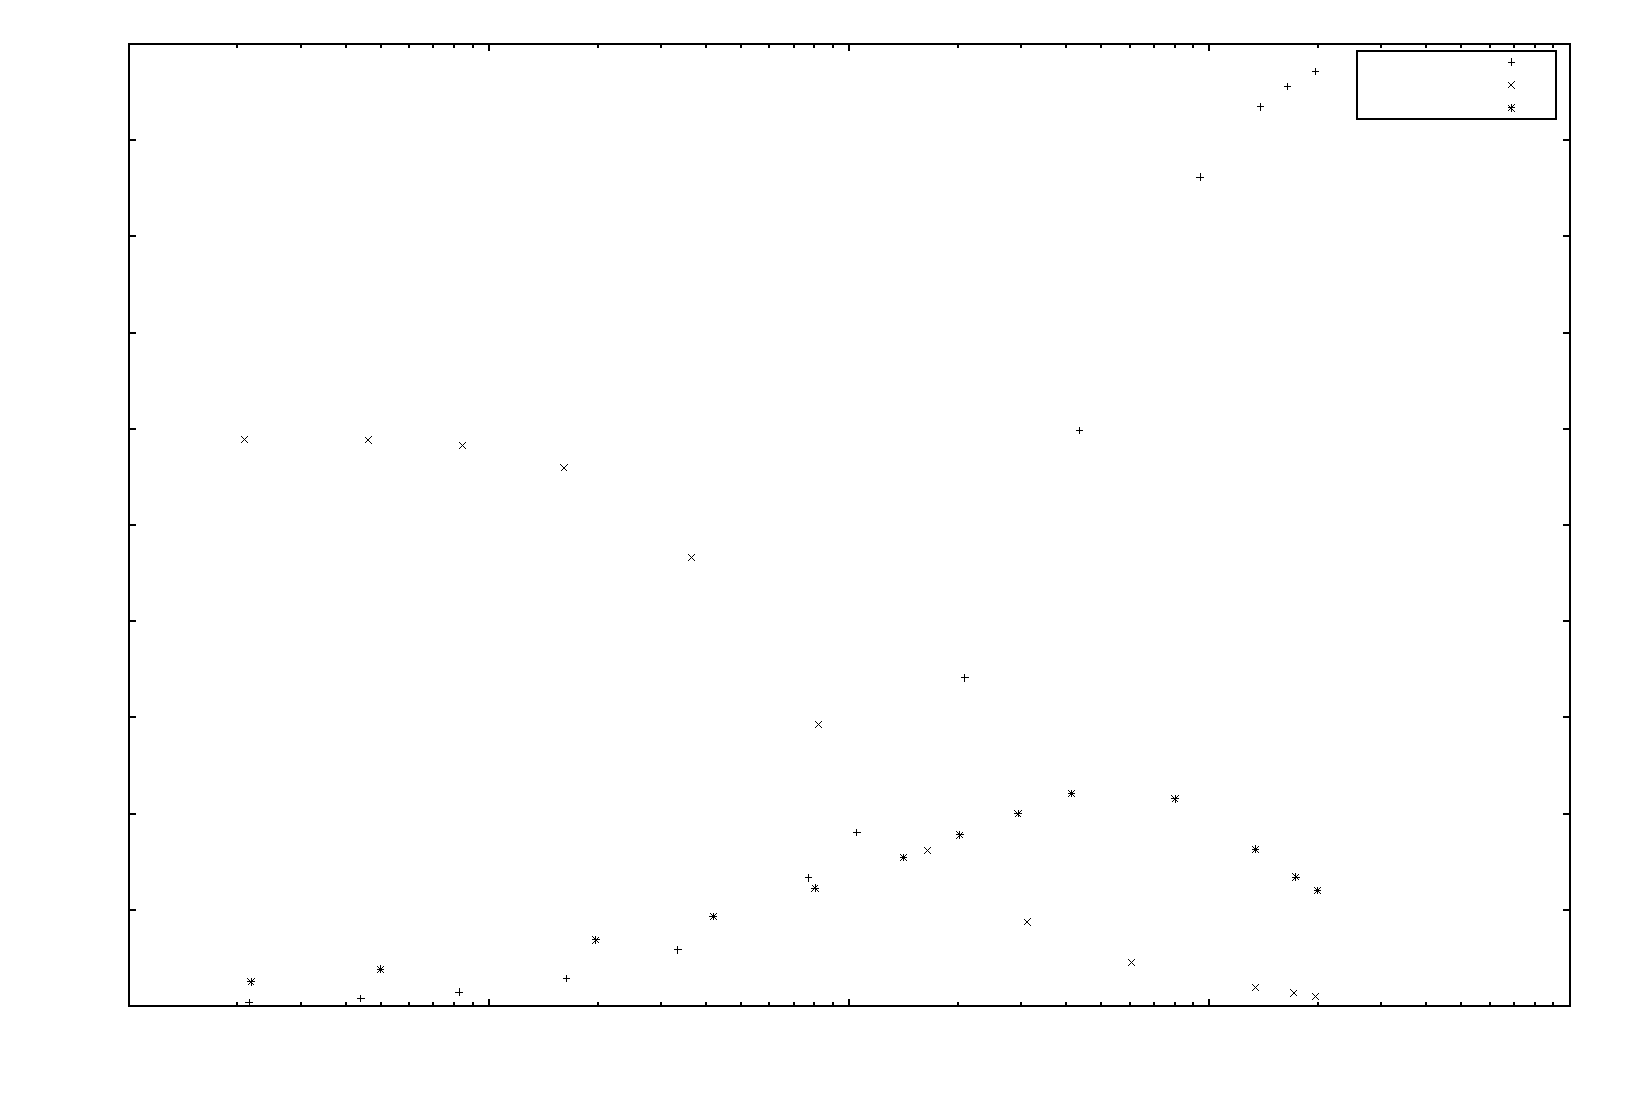
\includegraphics{plot-2}}%
    \gplfronttext
  \end{picture}%
\endgroup

\end{landscape}
\end{document}
